\chapter{Crash Course on Differential Equations}\label{app:de}

Differential equations (DEs) are fundamental tools for modeling dynamic systems and can be broadly categorized into \emph{ordinary differential equations} (ODEs), \emph{stochastic differential equations} (SDEs), and \emph{partial differential equations} (PDEs). 

ODEs describe how a system’s state changes over time according to a precise rule, so that knowing the starting point determines the future path exactly. SDEs add randomness to this evolution, modeling how noise or uncertainty influences the system’s behavior, making the outcome probabilistic rather than fixed. PDEs explain how functions depending on several variables, such as time and space, evolve together, capturing phenomena like heat spreading, waves moving, or \emph{the time evolution of probability densities in stochastic systems} (Spoiler: Fokker-Planck equation). These types of differential equations form a fundamental language for understanding how systems evolve over time and space under both deterministic and random influences.

In this chapter, we provide essential prerequisites on differential equations.

\clearpage
\newpage

\section{Foundation of Ordinary Differential Equations}

This section introduces the fundamental theory of ODEs, emphasizing the uniqueness of solutions given an initial condition. It also covers practical methods for solving ODEs using numerical solvers.


\subsection{Intuition of Ordinary Differential Equation}

The deterministic process is called an \emph{ordinary differential equation} (ODE). In the multivariate case, we consider systems of the form:
\begin{equation}\label{eq:general_ode}
    \frac{\diff \mathbf{x}(t)}{\diff t} = \mathbf{v}(\mathbf{x}(t), t),
\end{equation}
where $\mathbf{x}(t) \in \mathbb{R}^D$ is a vector-valued function representing the state of the system at time $t$, and $\mathbf{v}: \mathbb{R}^D \times \mathbb{R} \to \mathbb{R}^D$ is a vector field specifying the direction and magnitude of change at each point in space and time.


\paragraph{High-Level Intuition for Solving ODEs.}
\begin{figure}[th]
    \centering
    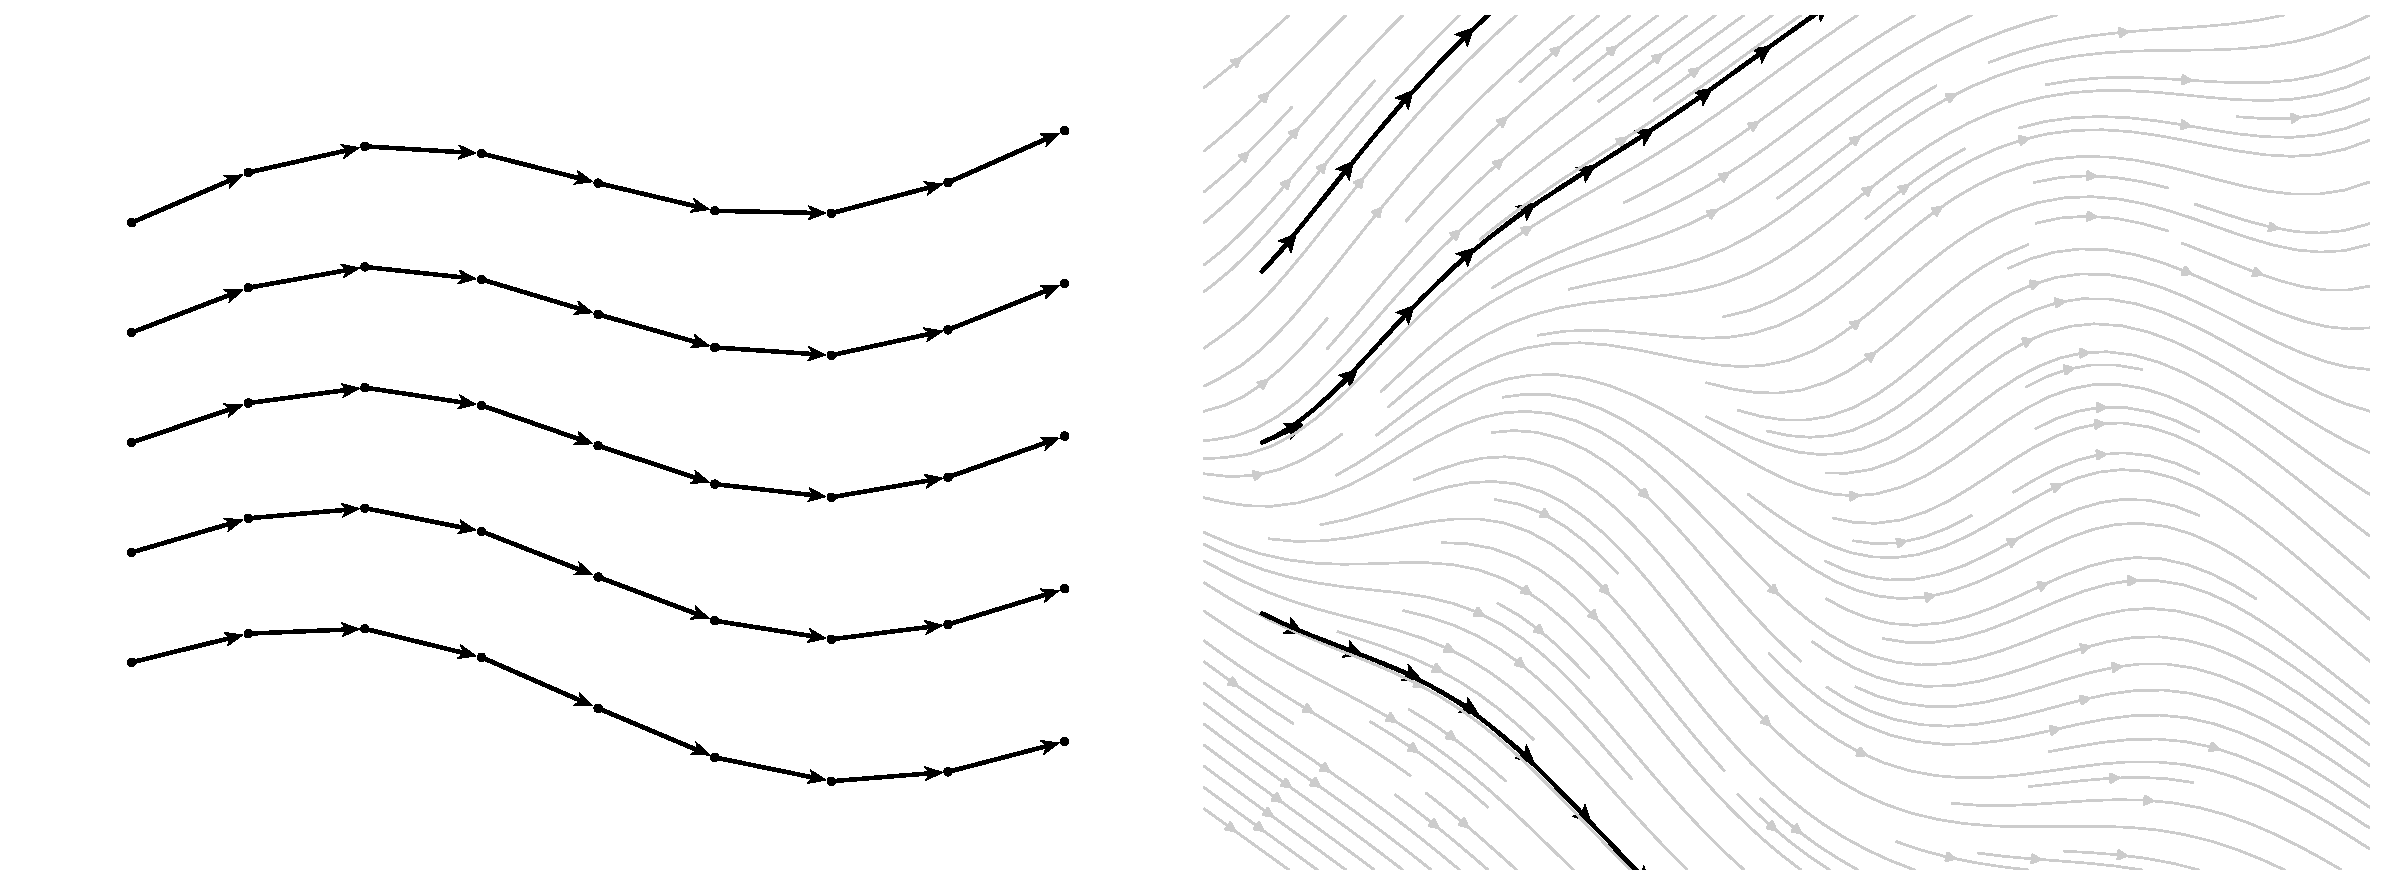
\includegraphics[width=\linewidth]{Images/PartE/discrete_vs_continuous_ode.pdf}
    \caption{\textbfs{ODE illustration.}  
A velocity field $\rvv(\rvx,t)$ assigns a drift vector at every point.  
A solution trajectory $\rvx(t)$ is a path whose tangent always matches the local drift.  
The left panel shows step-by-step solver updates (dots and arrows) approximating the path,  
while the right panel shows the exact trajectories (black) flowing consistently with the velocity field. Without specifying an initial state $\rvx(0)$, there are infinitely many trajectories whose instantaneous changes match the same velocity field.  
Once $\rvx(0)$ is fixed, however, the ODE determines a unique path $\rvx(t)$ that flows according to the drift.  
\figcredit{Created by the authors.}}
    \label{fig:ode-illustration}
\end{figure}

To build intuition, imagine the vector field $\mathbf{v}(\mathbf{x}, t)$ as a dynamic landscape of arrows that tells you how a point $\mathbf{x}$ should move at any given time $t$. Solving the differential equation means tracing out a curve $\mathbf{x}(t)$ through this field such that the tangent (i.e., the instantaneous velocity) of the curve at any point aligns with the vector given by $\mathbf{v}(\mathbf{x}(t), t)$.
\begin{itemize}
    \item \textbfs{Vector Field Perspective:} The function $\mathbf{v}(\mathbf{x}, t)$ defines how things should move: it gives the local ``instructions'' for motion or change.
    \item \textbfs{Trajectory Perspective:} The solution $\mathbf{x}(t)$ is a path that a particle would follow if it obeys the rule set by the vector field $\mathbf{v}$ at every instant.
\end{itemize}
Thus, solving an ODE is like placing a particle in a flow field and observing where it goes over time.

\subsection{Existence and Uniqueness of Ordinary Differential Equations}
So far, we have seen that solving an ODE means finding a path that follows the directions given by the vector field at every point. Intuitively, this is like tracing the trajectory of a particle as it moves along the flow defined by the velocities.

But this picture leads to an important question: 
\begin{question}
    If we pick a starting point, can we be sure there really is a path that follows these directions? And if there is, is that path unique, or could the particle suddenly jump onto a different trajectory?
\end{question}

Answering these questions is essential because it tells us whether the system’s behavior can be reliably predicted from its starting position.  
The \emph{Existence and Uniqueness Theorem} provides conditions on the vector field that guarantee exactly one path starting from any given initial point.  
This ensures the solution behaves consistently and forms a cornerstone of the theory of ODEs.  


\paragraph{Local (in Time) Existence and Uniqueness Theorem.}


Below, we state a \emph{local} version of the theorem, which asserts existence and uniqueness of a solution in a neighborhood of the initial time for a given initial condition.

\thmp{Local Existence and Uniqueness}{ode-local}{
Let $\mathbf{v}(\mathbf{x}, t)$ be a continuous function with respect to $\mathbf{x}$ and $t$ in a domain $D \subseteq \mathbb{R}^D \times \mathbb{R}$. If $\mathbf{v}$ satisfies the Lipschitz condition with respect to $\mathbf{x}$:
\[
\|\mathbf{v}(\mathbf{x}_1, t) - \mathbf{v}(\mathbf{x}_2, t)\| \leq L \|\mathbf{x}_1 - \mathbf{x}_2\| \quad \forall (\mathbf{x}_1, t), (\mathbf{x}_2, t) \in D,
\]
where $L > 0$ is a constant, then for every initial condition $\mathbf{x}(t_0) = \mathbf{x}_0$, there exists a unique solution $\mathbf{x}(t)$ to \Cref{eq:general_ode} defined on some interval $[t_0 - \delta, t_0 + \delta]$.}{(Proof Outline) The Existence and Uniqueness Theorem can be demonstrated constructively using the Picard-Lindel\"of iteration method. The method generates a sequence of functions $\{\mathbf{x}_n(t)\}$ that converges to the solution $\mathbf{x}(t)$. The iteration is defined as:
\[
\mathbf{x}_{n+1}(t) = \mathbf{x}_0 + \int_{t_0}^t \mathbf{v}(\mathbf{x}_n(s), s) \diff s.
\]
\begin{itemize}
    \item Start with an initial guess $\mathbf{x}_0(t) = \mathbf{x}_0$.
    \item Iteratively refine $\mathbf{x}_n(t)$ using the integral form.
    \item Convergence is guaranteed under the Lipschitz condition by applying Contraction Mapping Theorem.
\end{itemize}
}
The essence of the proof is rooted in the Picard–Lindelöf iteration method, whose core idea is also leveraged in \Cref{sec:picard} to accelerate the sampling process of diffusion models.


\paragraph{Global (in Time) Existence and Uniqueness Theorem.}
While the Local Existence and Uniqueness Theorem guarantees the existence of solutions on a small time interval, the ``global (in time) existence and uniqueness theorem'' extends this result to the entire interval $[t_0, T]$ under additional regularity conditions. A well-known result in this category is the \emph{Carathéodory theorem}, which ensures the global existence and uniqueness of solutions to ODEs under two key assumptions: local Lipschitz continuity in the state variable and a linear growth bound.

\begin{enumerate}[label=(\roman*)]
    \item \textbfs{Local Lipschitz condition in $\mathbf{x}$:} There exists a function $\mathrm{Lip}(t)$, integrable on $[0, T]$, such that for all $\mathbf{x}_1, \mathbf{x}_2 \in \mathbb{R}^D$,
    \[
    \|\rvv(\mathbf{x}_1, t) - \rvv(\mathbf{x}_2, t)\| \leq \mathrm{Lip}(t) \|\mathbf{x}_1 - \mathbf{x}_2\|.
    \]
    
    \item \textbfs{Linear growth condition:} There exists a function $M(t)$, integrable on $[0, T]$, such that for all $\mathbf{x} \in \mathbb{R}^D$,
    \[
    \|\rvv(\mathbf{x}, t)\| \leq M(t)(1 + \|\mathbf{x}\|).
    \]
\end{enumerate}
We refer the reader to \citep{reid1971ordinary} for a comprehensive discussion of the assumptions, formal statement, and detailed proof of the theorem.

\rmkb{To apply these theorems to the probability flow ODE in diffusion models (see \Cref{eq:prob_ode_gt}), it may be necessary to impose additional assumptions, such as conditions (i) and (ii), on the score function $\nabla_\rvx \log p_t(\rvx)$. These assumptions can be reasonably accepted without further justification by readers not focused on technical details.
}

In summary, when an initial condition is given to an ODE defined by a time-dependent velocity field, the trajectory of the particle flow is uniquely determined.

\paragraph{Uniqueness Implies Non-Intersection of Solutions} The uniqueness of solutions in ODEs, as guaranteed by the Local Existence and Uniqueness Theorem, implies a fundamental property: two different solution trajectories, starting from different initial conditions, cannot cross each other. This reflects the deterministic nature of ODEs, ensuring that each state evolves along a unique path. The following corollary formalizes this result.


\corp{Non-Intersection of Solutions}{
Consider two solutions $\rvx_1(t)$ and $\rvx_2(t)$ to the ODE
\[
\frac{\diff \rvx(t)}{\diff t} = \rvv\left(\rvx(t),t\right), \quad t \in [0,T].
\]
Suppose they have distinct initial values $\rvx_1(0) \neq \rvx_2(0)$. Then, these solutions do not intersect on $[0,T]$, i.e.,
\[
\rvx_1(t) \neq \rvx_2(t) \quad \text{for all } t \in [0,T].
\]
}{Assume, for the sake of contradiction, that there exists some $t^* \in (0,T]$ such that
\[
\mathbf{x}_1(t^*) = \mathbf{x}_2(t^*).
\]
Define the first time at which the two solutions meet as
\[
t_0 := \inf \{ t \in [0,T]|\mathbf{x}_1(t) = \mathbf{x}_2(t) \}.
\]
Since $\mathbf{x}_1(0) \neq \mathbf{x}_2(0)$ and $t^*$ is contained in this set, it follows that $t_0 > 0$. By continuity of $\mathbf{x}_1$ and $\mathbf{x}_2$, we have
\[
\mathbf{x}_1(t_0) = \mathbf{x}_2(t_0).
\]

Consider the initial value problem
\[
\frac{\mathrm{d}\mathbf{x}(t)}{\mathrm{d}t} = \mathbf{v}(\mathbf{x}(t), t), \quad \mathbf{x}(t_0) = \mathbf{x}_1(t_0).
\]
By the uniqueness theorem for ODEs, both $\mathbf{x}_1$ and $\mathbf{x}_2$ must coincide on the interval $[t_0, T]$. Applying uniqueness backward in time similarly implies that the two solutions coincide on $[0, t_0]$.
Therefore, the solutions satisfy
\[
\mathbf{x}_1(t) = \mathbf{x}_2(t) \quad \text{for all } t \in [0, T],
\]
which contradicts the assumption that $\mathbf{x}_1(0) \neq \mathbf{x}_2(0)$. Hence, we conclude that
\[
\mathbf{x}_1(t) \neq \mathbf{x}_2(t) \quad \text{for all } t \in [0, T].
\]

}

By guaranteeing non-intersecting solution paths, this theorem offers hidden yet crucial support for the flow map model (see \Cref{ch:distillation,ch:fast-scratch}).



\subsection{Exponential Integration Factor}\label{app:exp-int-factor}
Even an ODE determined by a general time-varying velocity $\rvv$ does not admit a closed-form solution, in some special cases, we can solve them analytically or by reducing its formulation to a better structural one.  
\paragraph{An Illustrative Example.}
Consider the following linear scalar ODE:
\[
\frac{\diff \rvx(t)}{\diff t} = L(t)\rvx(t),
\]
where $L(t) \in \mathbb{R}$ is a continuous function. This equation is solvable in closed form, and its solution is well known (for any $s$ and $t$):
\[
\rvx(t) = \rvx(s) \cdot \exp\left( \int_s^t L(\tau) \,\diff \tau \right).
\]
This formula demonstrates how the solution evolves according to an exponential factor that accumulates the effect of the time-dependent coefficient $L(t)$. This motivates the use of \emph{exponential integration factors}:
\begin{align}\label{eq:exp-int-factor}
    \mathcal{E}(s \shortrightarrow t) := \exp\left( \int_s^t L(\tau)\diff \tau \right),
\end{align}
especially in more general settings where the dynamics include both linear and nonlinear components.



\paragraph{Semilinear ODEs and Exponential Integration Factors.}
We now consider a broader class of ODEs known as \emph{semilinear} ODEs. These equations separate the dynamics into a linear part (in the state variable) and a nonlinear remainder:
\begin{align}\label{eq:semilinear-ode}
    \frac{\diff \rvx(t)}{\diff t} = L(t)\rvx(t) + \rmN(\rvx(t), t),
\end{align}
where $\rvx(t) \in \mathbb{R}^D$ is the state vector, $L(t)$ is a scalar-valued continuous function, and $\rmN: \mathbb{R}^D \times [0,T] \to \mathbb{R}^D$ is a nonlinear vector field. This semilinear structure arises naturally in many physical and engineering systems. In particular, it also appears in the probability flow ODE formulation of diffusion models (see \Cref{eq:prob_ode_gt}). Recognizing this structure enables the use of exponential integration factors, which not only simplify analysis but also improve numerical stability. Specifically, this technique plays a central role in the design of fast diffusion ODE solvers (see \Cref{ch:solvers}).


\subparagraph{Step 1: Isolate the Non-Linear Term via an Integration Factor.}
Observing that we can isolate the nonlinear part by subtracting the linear drift from the semiliner ODE in \Cref{eq:semilinear-ode}:
\[
\frac{\diff \rvx(t)}{\diff t} - L(t)\rvx(t) = \rmN(\rvx(t), t).
\]
To absorb the linear term, we multiply both sides by the inverse integration factor:
\[
\mathcal{E}^{-1}(s \shortrightarrow t) = \exp\left(-\int_s^t L(\tau)\diff \tau \right).
\]
Now apply the product rule to the left-hand side:
\begin{align*}
\mathcal{E}^{-1}(s \shortrightarrow t) \left( \frac{\diff \rvx(t)}{\diff t} - L(t)\rvx(t) \right)
&= \frac{\diff}{\diff t} \left[ \mathcal{E}^{-1}(s \shortrightarrow t) \rvx(t) \right].
\end{align*}
Hence, the equation becomes:
\[
\frac{\diff}{\diff t} \left[ \mathcal{E}^{-1}(s \shortrightarrow t) \rvx(t) \right]
= \mathcal{E}^{-1}(s \shortrightarrow t) \rmN(\rvx(t), t).
\]

This transformation simplifies the original equation by isolating the nonlinear component, allowing us to focus entirely on the nonlinear dynamics in a transformed coordinate system.

\subparagraph{Step 2: Integrate Over Time.}
We now integrate both sides from $s$ to $t$:
\[
\int_s^t \frac{\diff}{\diff \tau} \left[ \mathcal{E}^{-1}(s \shortrightarrow \tau) \rvx(\tau) \right] \diff \tau
= \int_s^t \mathcal{E}^{-1}(s \shortrightarrow \tau) \rmN(\rvx(\tau), \tau)\diff \tau.
\]
The left-hand side is simply the difference of the transformed variable evaluated at $t$ and $s$:
\[
\mathcal{E}^{-1}(s \shortrightarrow t) \rvx(t) - \rvx(s).
\]
Hence, we obtain:
\[
\mathcal{E}^{-1}(s \shortrightarrow t) \rvx(t)
= \rvx(s) + \int_s^t \mathcal{E}^{-1}(s \shortrightarrow \tau) \rmN(\rvx(\tau), \tau)\diff \tau.
\]

\subparagraph{Step 3: Solve for $\rvx(t)$.}
Multiplying both sides by the exponential flow $\mathcal{E}(s \shortrightarrow t)$ gives the solution:
\begin{align}\label{eq:exp-int-factor-integration}
    \rvx(t) = \underbrace{\mathcal{E}(s \shortrightarrow t)  \rvx(s)}_{\text{linear part}} + \underbrace{\int_s^t \mathcal{E}(\tau \shortrightarrow t) \rmN(\rvx(\tau), \tau)\diff \tau}_{\text{nonlinear part}} .
\end{align}

The solution naturally separates into a linear and a nonlinear component. Exponential integrators exploit this structure by solving the linear part in exactly closed form and discretizing only the nonlinear residual. This ensures that the step size is dictated by the nonlinear dynamics rather than by the potentially large linear coefficient, yielding updates that are both stable and accurate even with fewer steps (see the comparison between the exponential Euler update \Cref{eq:exp-euler-step} and the vanilla Euler update \Cref{eq:euler-step}).  






\subsection{Numerical Solvers of Ordinary Differential Equations}\label{app:de-solver}
We consider the ODE in \Cref{eq:general_ode} with an initial condition $\mathbf{x}(0)$. Solving this ODE involves finding a continuous trajectory $\mathbf{x}(t)$ that satisfies the equation for all $t \in [0, T]$. Ideally, a closed-form solution is desirable, though it is rarely attainable in practice.

A useful perspective is to rewrite the ODE in its integral form:
\begin{equation}
\label{eq:integral_form}
\mathbf{x}(t) = \mathbf{x}(0) + \int_0^t \mathbf{v}(\mathbf{x}(\tau), \tau)\diff \tau,
\end{equation}
which expresses the solution as the initial state plus the accumulated effect of the velocity over time. However, the integral is often intractable due to the nonlinear and time-dependent nature of $\mathbf{v}$, making closed-form solutions unavailable.

In such cases, we turn to \emph{numerical methods}, which discretize time and iteratively approximate $\mathbf{x}(t)$. Common approaches include Euler's method, Runge–Kutta methods, and specialized integrators for stiff systems. These methods simulate the system step by step, providing practical approximations of the true trajectory.

\rmkb{When $\mathbf{v}$ takes the semilinear form in \Cref{eq:semilinear-ode}, the solution admits an integral representation involving an exponential integration factor (\Cref{eq:exp-int-factor-integration}), which separates the linear and nonlinear components. This structure enables efficient numerical solvers that focus solely on approximating the nonlinear term, reducing computational complexity and motivating tailored algorithms (see \Cref{ch:solvers}).}




\paragraph{Key Concepts.}
Numerical solvers approximate the continuous dynamics of ODEs by discretizing time and estimating the state using the slope $\mathbf{v}$ of the ODE. This involves:
\begin{itemize}
    \item \textbfs{Discretization:} Partition the time domain into discrete steps $t_0, t_1, \dots, t_n$.
    \item \textbfs{Step Size:} The interval $\Delta t_i = t_{i+1} - t_i$ is called the step size.
    \item \textbfs{Approximation:} The solution at each step is estimated numerically; the accuracy depends on the step size and the method used.
    \item \textbfs{Error Control:} Errors from discretization and approximation are monitored and controlled.
\end{itemize}

\paragraph{High-Level Categorization of Numerical Solvers.}
ODE solvers can be broadly categorized as:
\begin{itemize}
    \item \textbfs{Time-Stepping Methods:} These methods advance the solution step by step, e.g., explicit/implicit Euler, Runge-Kutta.
    \item \textbfs{Time-Parallel Methods:} These methods leverage parallelism to compute solutions over different time intervals simultaneously, useful for large-scale problems.
\end{itemize}

\paragraph{Common Numerical Solvers.} Among these, Euler, Heun, and Runge--Kutta are \emph{single-step methods}, since 
each update uses only the current state $(t_n,\mathbf{x}_n)$. 
In contrast, \emph{multi-step methods} (such as Adams--Bashforth or Adams--Moulton) 
compute $\mathbf{x}_{n+1}$ using not only the current state $\mathbf{x}_n$ but also 
several previous values $\mathbf{x}_{n-1}, \mathbf{x}_{n-2}, \dots$. 
They save work by reusing past information (history anchors) instead of re-evaluating 
everything within the current step. 
Such methods are not covered here, though related schemes (e.g., Adams--Bashforth, 
discussed in \Cref{sec:exponential,sec:dpm++}) also exploit multiple past states. 

Picard iteration, on the other hand, is of a different nature: it serves as a 
theoretical fixed-point construction, whose idea will be revisited in 
\Cref{sec:picard}.


\subparagraph{Euler's Method.}
Euler's method is the simplest time-stepping scheme:
\[
\mathbf{x}_{n+1} = \mathbf{x}_n + h \mathbf{v}(\mathbf{x}_n, t_n),
\]
where $h$ is the step size. It has first-order accuracy: local error $\mathcal{O}(h^2)$, global error $\mathcal{O}(h)$. While easy to implement, it requires small $h$ for stability and accuracy.

\subparagraph{Heun's Method (Improved Euler).}
Heun's method is a second-order predictor-corrector scheme:
\begin{align*}
\text{Predict:} \quad &\mathbf{x}_{\text{pred}} = \mathbf{x}_n + h \mathbf{v}(\mathbf{x}_n, t_n), \\
\text{Correct:} \quad &\mathbf{x}_{n+1} = \mathbf{x}_n + \frac{h}{2} \big(\mathbf{v}(\mathbf{x}_n, t_n) + \mathbf{v}(\mathbf{x}_{\text{pred}}, t_n + h)\big).
\end{align*}
It achieves local error $\mathcal{O}(h^3)$ and global error $\mathcal{O}(h^2)$. \citet{karras2022elucidating} advocate Heun's method for solving ODEs in diffusion models, though higher-order methods such as DPM-Solvers (see \Cref{sec:dpm,sec:dpm++}) typically yield better performance.

\subparagraph{Runge-Kutta Methods.}
Runge-Kutta (RK) methods generalize Euler by using weighted averages of intermediate slopes. The fourth-order method (RK4) is a standard choice:
\begin{align*}
\mathbf{k}_1 &= \mathbf{v}(\mathbf{x}_n, t_n), \\
\mathbf{k}_2 &= \mathbf{v}(\mathbf{x}_n + \tfrac{h}{2} \mathbf{k}_1, t_n + \tfrac{h}{2}), \\
\mathbf{k}_3 &= \mathbf{v}(\mathbf{x}_n + \tfrac{h}{2} \mathbf{k}_2, t_n + \tfrac{h}{2}), \\
\mathbf{k}_4 &= \mathbf{v}(\mathbf{x}_n + h \mathbf{k}_3, t_n + h), \\
\mathbf{x}_{n+1} &= \mathbf{x}_n + \tfrac{h}{6}(\mathbf{k}_1 + 2\mathbf{k}_2 + 2\mathbf{k}_3 + \mathbf{k}_4).
\end{align*}
RK4 balances accuracy and cost, making it widely used. DPM-Solver builds on similar ideas to achieve higher-order accurate integration tailored to diffusion models, leveraging their semilinear structure (see \citep{lu2022dpm}'s Appendix B.6 for a comparison).

\subparagraph{Picard Iteration.}
Picard iteration refines successive approximations to the solution via:
\[
\mathbf{x}^{(k+1)}(t)
= \mathbf{x}(0) + \int_0^t \mathbf{v}\!\big(\mathbf{x}^{(k)}(s), s\big) \diff s,
\]
starting from an initial guess function
$\mathbf{x}^{(0)}(t)$ with $\mathbf{x}^{(0)}(0)=\mathbf{x}(0)$. While theoretically foundational, Picard iteration often converges slowly due to its strong dependence on the initial guess. Moreover, each iteration involves computing an integral over time, which can be computationally expensive.



\paragraph{Solving ODEs in Forward and Reverse Time.}
So far, we have considered solving the ODE in \Cref{eq:general_ode} \emph{forward in time}, evolving the solution from an initial condition $\rvx(0)$ to later times $t > 0$.

In contrast, \emph{reverse-time} integration computes the solution by stepping backward from a terminal condition $\rvx(T)$ toward earlier times $t < T$. Reparameterizing time as $T - t$ transforms the ODE into:
\[
\frac{\diff \mathbf{x}(t)}{\diff t}
= -\,\mathbf{v}\big(\mathbf{x}(t),\,T - t\big),
\qquad \mathbf{x}(0)=\mathbf{x}(T).
\]
Reverse-time integration applies the same methods as forward-time integration, 
but on a decreasing time grid. With Euler and step size $h>0$, starting from 
$t_0=T$ with $\mathbf{x}_0=\mathbf{x}(T)$, the updates are
\[
t_{n+1}=t_n-h, \quad 
\mathbf{x}_{n+1}=\mathbf{x}_n - h\,\mathbf{v}(\mathbf{x}_n,t_n).
\]
Care must be taken to ensure numerical stability, especially for stiff problems (i.e., when some components of the state vector evolve much faster than others, requiring very small time steps for stable integration), as commonly encountered in PF-ODE sampling for diffusion models.

While time reversal for ODEs is theoretically straightforward, as it only requires a reparameterization of time due to the bijective mapping between $\rvx(0)$ and $\rvx(T)$, this does not hold for SDEs. Their intrinsic randomness precludes direct time reversal, a point we elaborate on in the next section.

\newpage
\clearpage


\section{Foundation of Stochastic Differential Equations}\label{app:sde-intro}

Stochastic Differential Equations (SDEs) are an extension of ordinary differential equations (ODEs) that incorporate randomness, providing a mathematical framework for modeling systems affected by uncertainty. This chapter introduces SDEs, beginning with the discretization of ODEs, extending to the discretization of SDEs, and culminating in a discussion of general SDEs, including Ito's calculus and Ito's formula.

\subsection{From ODEs to SDEs: An Intuitive Introduction}
Let us begin with a ODE describing the deterministic evolution of a state variable $ \rvx(t) \in \mathbb{R}^D $:
\begin{equation}
    \frac{\diff\rvx(t)}{\diff t} = \rvf(\rvx(t), t), \quad \rvx(0) = \rvx_0.
    \label{eq:ode}
\end{equation}
Here, $ \rvf: \mathbb{R}^D \times [0,T] \rightarrow \mathbb{R}^D $ is a time-dependent velocity field that governs the dynamics of $ \rvx(t) $. The solution to this ODE is a smooth trajectory $ t \mapsto \rvx(t) $, fully determined by the initial condition $ \rvx_0 $.

\paragraph{Discretization Perspective.} To build intuition, consider an Euler discretization of \Cref{eq:ode} over small time steps $ \Delta t $:
\begin{equation*}
    \rvx_{t+\Delta t} = \rvx_t + \rvf(\rvx_t, t) \Delta t.
\end{equation*}
This approximation becomes more accurate as $ \Delta t \to 0 $, converging (under standard regularity conditions on $ \rvf $) to the exact solution of the ODE.

\paragraph{Introducing Randomness: From ODE to SDE.} In many real-world systems, perfect knowledge of the dynamics is unrealistic. Noise, uncertainty, or unmodeled interactions may affect the evolution. To incorporate such randomness, we augment the ODE with a stochastic term:
\begin{equation}
    \rvx_{t+\Delta t} = \rvx_t + \rvf(\rvx_t, t)\Delta t + g(t)\sqrt{\Delta t} \cdot \bm{\epsilon}_t,
    \label{eq:euler-sde}
\end{equation}
where
\begin{itemize}
    \item $g: [0,T] \to \mathbb{R}$ is a diffusion coefficient (possibly dependent on both state and time, though here assumed time-dependent only),
    \item $\bm{\epsilon}_t \sim \mathcal{N}(\bm{0}, \rmI_D)$ are i.i.d. standard Gaussian vectors.
\end{itemize}

This modified update rule reflects not just deterministic drift, but also random perturbations scaled by $ \sqrt{\Delta t} $. The scaling ensures that the stochastic perturbation remains finite in the limit $ \Delta t \to 0 $. Importantly, this formulation gives rise to a \emph{continuous-time stochastic process} as $ \Delta t \to 0 $, which leads us to the framework of SDE.

\paragraph{Stochastic Differential Equations.}
Formally, the limit of the discrete update~\Cref{eq:euler-sde} as $ \Delta t \to 0 $ defines the SDE:
\begin{equation}
    \diff \rvx(t) = \rvf(\rvx(t), t)\diff t + g(t) \diff \rvw(t).
    \label{eq:sde}
\end{equation}
Here, $ \rvw(t) \in \mathbb{R}^D $ is a \emph{Wiener process} (standard Brownian motion), a continuous-time stochastic process characterized by:
\begin{itemize}
    \item \textbfs{Initial State:} $ \rvw(0) = 0 $ almost surely;
    \item \textbfs{Independent Increments:}  for $ 0 \leq s < t $, the increment $ \rvw(t) - \rvw(s) $ is independent of the past;
    \item \textbfs{Gaussian Increments:} 
    \begin{align}\label{eq:wiener-gaussian}
        \rvw(t) - \rvw(s) \sim \mathcal{N}\bigl(\bm{0}, (t - s)\rmI_D \bigr)
    \end{align}
    \item \textbfs{Continuity:} Sample paths $ t \mapsto \rvw(t) $ are almost surely continuous but nowhere differentiable.
\end{itemize}
In addition, the notation
\[
\diff \rvw(t) := \rvw(t + \diff t) - \rvw(t)
\]
is often used to denote the infinitesimal increment of the Wiener process. 

While suggestive, this notation is heuristic and should not be interpreted as a classical differential (e.g., in the Riemann or Lebesgue sense), since Brownian paths are almost surely nowhere differentiable. Instead, it serves as a formal shorthand to express the Gaussian increments property:
\[
\diff \rvw(t) \sim \mathcal{N}(0, \diff t\, \mathrm{I}_D),
\]
meaning that over an infinitesimal time interval of length $ \diff t $, the increment of the Wiener process behaves like a Gaussian random variable with zero mean and covariance $ \diff t\, \mathrm{I}_D $.




\subsection{Further Explanation of \Cref{eq:sde}}
The SDE in \Cref{eq:sde} should be understood in its \emph{integral form}:
\begin{align}\label{eq:sde-integral-form}
    \rvx(t) = \rvx(0) + \int_0^t \rvf(\rvx(s), s) \diff s + \int_0^t g(s) \diff \rvw(s),
\end{align}
interpreted in the \emph{Itô sense}.
Here, the first term is a classical (Riemann or Lebesgue) integral representing the accumulated deterministic drift, while the second term is an \emph{Itô stochastic integral}, which integrates with respect to the Wiener process $ \rvw(t) $. We do not provide a full rigorous construction of the Itô integral, but offer the following intuition.


\paragraph{Intuition for It\^o Integration.}
The It\^o integral can be understood as the limit of discrete sums of
the form\footnote{For square-integrable integrands, this convergence holds in the $L^2$ sense (mean-square), which in turn implies convergence in probability. The $L^2$ viewpoint is natural because it connects directly to It\^o's isometry, the key identity underlying the standard and rigorous construction of the It\^o integral. This isometry links stochastic integrals to standard integrals in expectation ($\E\bigl[\bigl\|\int_0^T \bm{\psi}(t)\,\mathrm{d}\rvw_t \bigr\|^2\bigr] = \E\bigl[\int_0^T \|\bm{\psi}(t)\|_F^2\,\mathrm{d}t\bigr]$ with Frobenius norm
$\|\bm{\psi}(t)\|_F^2$); we state and use it in \Cref{subsec:rigorous-proof-linear-sde}.}
\[
\sum_i g(t_i)\bigl(w(t_{i+1})-w(t_i)\bigr),
\]
where the integrand $g(t)$ is evaluated at the \emph{left} endpoint
$t_i$ of each subinterval. As the partition becomes finer, these sums
converge to the It\^o integral. The left-point evaluation rule is what
distinguishes It\^o integration from classical integrals, which may use
midpoints or other evaluation rules. Because Brownian paths are
continuous yet almost surely nowhere differentiable, classical
integration does not directly apply. The It\^o integral handles this
irregularity and captures the cumulative effect of stochastic
fluctuations over time.

\paragraph{Use of Differential Notation.}
Expressions such as $ \diff \rvx(t) $, $ \diff t $, and $ \diff \rvw(t) $ are not classical differentials. Instead, they are formal notations representing infinitesimal increments of the respective processes. While heuristic, they are widely used for their convenience in expressing SDEs analogously to ODEs and facilitate formal manipulations within Itô calculus.

How Itô calculus is applied in diffusion models will be explained in \Cref{app:Ito}.


\paragraph{Comparison with ODEs.}
In ODEs, e.g.,
\[
\frac{\diff \rvx(t)}{\diff t} = \rvf(\rvx(t), t),
\]
the integral form
\[
\rvx(t) = \rvx(0) + \int_0^t \rvf(\rvx(\tau), \tau) \diff \tau
\]
is justified by the \emph{Fundamental Theorem of Calculus}, which ensures that differentiable functions can be recovered from their derivatives.

By contrast, in SDEs such as \Cref{eq:sde}, there is no direct analog of this theorem because Brownian motion lacks differentiability, and stochastic integrals do not follow the classical chain rule. Instead, Itô calculus introduces alternative tools (e.g., Itô's lemma) to analyze and manipulate stochastic dynamics.

Thus, while the differential notation for SDEs is compact and intuitive, a rigorous understanding depends on interpreting them via their integral formulation using Itô integrals.



\subsection{A Numerical Solver for SDE.} Like ODEs, the SDE in \Cref{eq:sde} admits a unique solution\footnote{The solution is in the \emph{strong} sense, meaning that $\mathbf{x}(t)$ satisfies the SDE in its integral form (see \Cref{eq:sde-integral-form}) with respect to the given Brownian motion $\mathbf{w}(t)$ on a fixed probability space. We omit the detailed technical definitions here.} if $\mathbf{f}(\cdot, t)$ and $g(\cdot)$ satisfy some smoothness conditions: $\mathbf{f}(\cdot, t)$ is Lipschitz and of linear growth in $\mathbf{x}$, and $g(\cdot)$ is square integrable.


For general SDEs as in \Cref{eq:sde}, closed-form solutions are generally unavailable, so numerical methods are necessary. A common approach is the \emph{Euler–Maruyama method}, which generalizes Euler’s method for ODEs and, indeed, we have already seen it in \Cref{eq:euler-sde}. It approximates the drift term $\rvf(\rvx(t), t)$ over a time step $\Delta t$ and simulates the stochastic noise $g(t) \diff \rvw(t)$ using Gaussian increments $\sqrt{\Delta t} \, \boldsymbol{\epsilon}_t$ with $\boldsymbol{\epsilon}_t \sim \mathcal{N}(\mathbf{0}, \mathbf{I})$. 

Later, in \Cref{subsec:rigorous-proof-linear-sde}, we will see that a linear SDE admits a closed-form solution.


